\chapter{Directional data}
\label{ch:directional}

Strike and dip, azimuth and elevation, latitude and longitude,
$\ldots$ \textit{directional data} are ubiquitous in the Earth
Sciences. Just like the compositional data discussed in
chapter~\ref{ch:compositional}, the statistical analysis of these
directional data is fraught with dangers.

\section{Circular data}
\label{sec:circular}

Consider the following dataset of directions (in degrees) of thirty
glacial striations from Madagascar:

\begin{center}
\begin{tabular}{ccccccccccccccc}
44 & 51 & 79 & 65 & 27 & 31 & 4 & 355 & 22 & 352 & 287 & 7 & 287 & 339 & 0 \\
276 & 342 & 355 & 334 & 296 & 7 & 17 & 351 & 349 & 37 & 339 & 40 & 324 & 325 & 334\\
\end{tabular}
\end{center}

These values span a range from 0$^{\circ}$ and 360$^{\circ}$, where
$0^{\circ}=360^{\circ}$. Plotting the data on a circle:

\noindent\begin{minipage}[t][][b]{.25\textwidth}
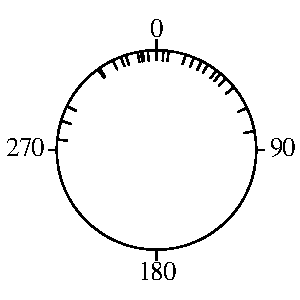
\includegraphics[width=\textwidth]{../figures/circle1.pdf}\medskip
\end{minipage}
\begin{minipage}[t][][t]{.75\textwidth}
  \captionof{figure}{The directions of 30~glacial striations. The
    values are roughly centred around zero but exhibit significant
    scatter, from the northwest (276$^\circ$) to the northeast
    (79$^\circ$).\medskip}
  \label{fig:circle1}
\end{minipage}

Computing the arithmetic mean of these angles yields a value of
189.2$^{\circ}$. This is a nonsensical result:

\noindent\begin{minipage}[t][][b]{.25\textwidth}
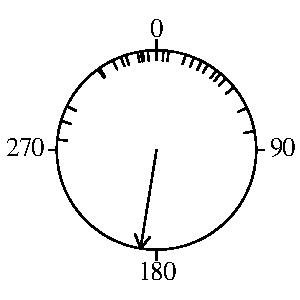
\includegraphics[width=\textwidth]{../figures/circle2.pdf}\medskip
\end{minipage}
\begin{minipage}[t][][t]{.75\textwidth}
  \captionof{figure}{The same glacial striation data of
    Figure~\ref{fig:circle1}, with their arithmetic mean shown as an
    arrow. Even though the individual striations are all pointing
    north, their arithmetic mean is pointing in exactly the opposite
    direction.\medskip}
  \label{fig:circle2}
\end{minipage}

The problem is that directional data are `wrapped around' a circle.
The difference between $1^{\circ}$ and $359^{\circ}$ is not
$358^{\circ}$ but $2^{\circ}$. So the usual rules of arithmetic do not
apply to angular measurements. Better results for the difference
between two angles $\theta$ and $\phi$ are obtained using the
following trigonometric relationship:
\begin{equation}
  d[\theta,\phi] =
  \arcsin\left( \sin[\theta] \cos[\phi] -
  \cos[\theta] \sin[\phi] \right)
  \label{eq:anglediff}
\end{equation}

Similarly, the mean of 1$^\circ$ and 359$^\circ$ should not be
180$^\circ$ but 0$^\circ$. A more sensible definition of the `mean
direction' is again obtained using trigonometry, by taking the
\textbf{vector sum} of all the component directions. For example, if
$\theta = \{\theta_1, \ldots, \theta_i, \ldots \theta_n \}$ are $n$
angles, then the resultant direction is obtained by summing the
horizontal and vertical components of unit vectors pointing in these
directions:
\begin{equation}
  \overline{\theta} = \mbox{arctan2}\left(
  \sum_{i=1}^{n}\sin[\theta_i],\sum_{i=1}^{n}\cos[\theta_i]
  \right)
  \label{eq:averagedirection}
\end{equation}

\noindent where
\begin{equation}
  \mbox{arctan2}(y,x) = 
  \begin{cases}
    \arctan(y/x) & \mbox{~if~} x>0 \mbox{~and} \\
    \arctan(y/x) \pm \pi & \mbox{~if~} x<0
  \end{cases}
\end{equation}

Applying this formula to the glacial striation data:

\noindent\begin{minipage}[t][][b]{.25\textwidth}
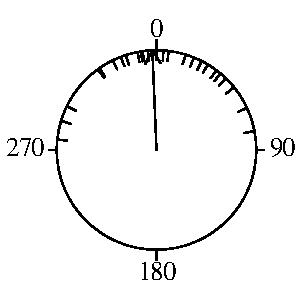
\includegraphics[width=\textwidth]{../figures/circle3.pdf}\medskip
\end{minipage}
\begin{minipage}[t][][t]{.75\textwidth}
  \captionof{figure}{The vector sum of the 30 glacial striation
    measurements points in a direction of 357.6$^\circ$, which is
    marked by the arrow and does a much better job at capturing the
    `central' direction than the arithmetic mean of
    Figure~\ref{fig:circle2} does.\medskip}
  \label{fig:circle3}
\end{minipage}

Dividing the length of the vector sum by the number of measurements
yields a new summary statistic, $\bar{R}$, which is shown as a thick
black arrow in Figure~\ref{fig:vectorsum}.
\begin{equation}
  \bar{R} = \sqrt{\left(\sum_{i=1}^{n} \sin[\theta_i]/n\right)^2 +
    \left( \sum_{i=1}^{n}\cos[\theta_i]/n \right)^2}
  \label{eq:circularR}
\end{equation}

\noindent\begin{minipage}[t][][b]{.45\textwidth}
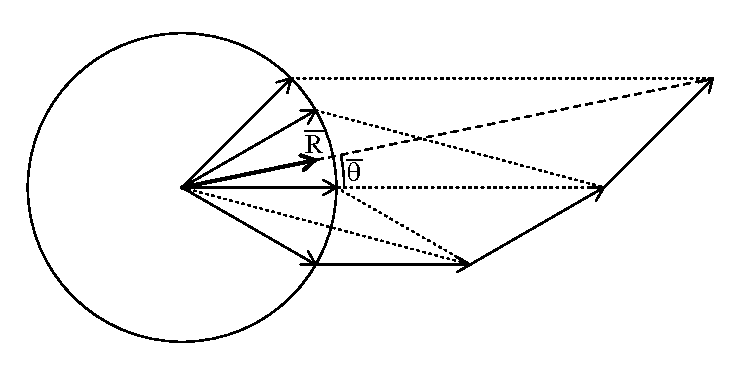
\includegraphics[width=\textwidth]{../figures/vectorsum.pdf}\medskip
\end{minipage}
\begin{minipage}[t][][t]{.55\textwidth}
  \captionof{figure}{An average direction (dashed line) is obtained by
    taking the vector sum of four angular measurements (thin black
    arrows).  Scaling by the number of measurements (thick black
    arrow) yields a measure of concentration ($0 \leq \bar{R} \leq
    1$), which increases in length with decreasing angular dispersion
    and vice versa.\medskip}
  \label{fig:vectorsum}
\end{minipage}

This arrow shortens with increasing scatter and so $\bar{R}$ is not a
dispersion parameter like the standard deviation, but a
\textit{concentration parameter}. To create a dispersion parameter, we
can use $\bar{R}$ to define the \textbf{circular standard deviation}:
\begin{equation}
  s_c = \sqrt{\ln(1/\bar{R}^2)}
  \label{eq:circularSD}
\end{equation}

In the extreme case where all the measurements point in the same
direction, $\bar{R} = 1$ and $s_c = 0$. If the data are evenly
distributed around the circle, then $\bar{R} = 0$ and $s_c = \infty$.

\noindent\begin{minipage}[t][][b]{.2\textwidth}
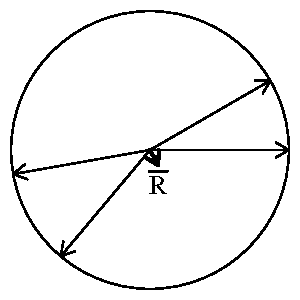
\includegraphics[width=\textwidth]{../figures/lowconcentration.pdf}\medskip
\end{minipage}
\begin{minipage}[t][][t]{.8\textwidth}
  \captionof{figure}{When the directional measurements are greatly
    dispersed, the normalised vector sum $\bar{R}$ is short
    ($\bar{R}=0.125$ in this example), and the circular standard
    deviation is large ($s_c=4.16$).\medskip}
  \label{fig:lowconcentration}
\end{minipage}

\section{Circular distributions}
\label{sec:circular-distributions}

The normal distribution is inappropriate for directional data, for the
same reason why it was inappropriate for compositional data: its tails
go from $-\infty$ to $+\infty$ and do not fit within the constrained
data space of the angles. The \textbf{von Mises distribution} does not
suffer from this problem:
\begin{equation}
  f(\theta|\mu,\kappa) \propto \exp[\kappa \cos(\theta-\mu)]
  \label{eq:vonMises}
\end{equation}

\noindent where $\mu$ is the location parameter (the mean angle) and
$\kappa$ is the concentration parameter. As the name suggests, large
$\kappa$-values correspond to narrow distributions, and small
$\kappa$-values to wide ones.

\noindent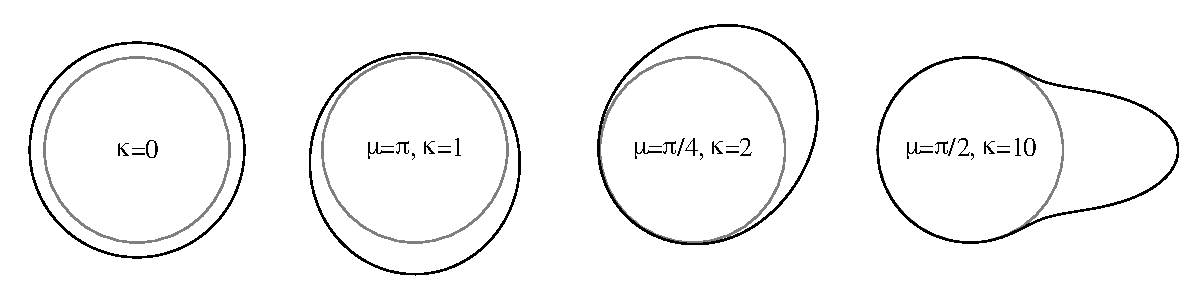
\includegraphics[width=\textwidth]{../figures/vonMises.pdf}
\begingroup \captionof{figure}{Four examples of the von Mises
  distribution with different values for the mean $\mu$ and the
  concentration parameter $\kappa$, wrapped around a (grey)
  circle. The probability density is proportional to the distance from
  the circle to the black line.\medskip}
\label{fig:vonMises}\endgroup

The parameter $\kappa$ is not easy to determine directly, but can be
estimated indirectly via the concentration parameter $\bar{R}$ and the
following approximation:
\begin{equation}
  \hat{\kappa} = \frac{\bar{R}(p+1-\bar{R}^2)}{1-\bar{R}^2}
  \label{eq:kappa}
\end{equation}

\noindent where $p$ marks the number of parameters, namely $p=1$ for
circular data and $p=2$ for spherical data
(Section~\ref{sec:spherical-distributions}).

\noindent\begin{minipage}[t][][b]{.3\textwidth}
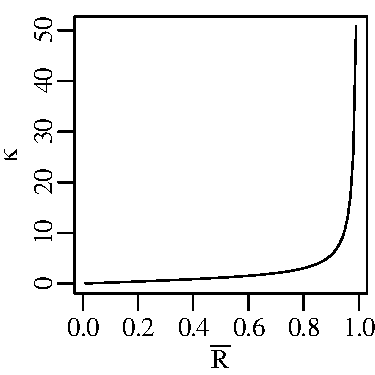
\includegraphics[width=\textwidth]{../figures/R2K.pdf}\medskip
\end{minipage}
\begin{minipage}[t][][t]{.7\textwidth}
  \captionof{figure}{$\bar{R}$ and $\kappa$ are two concentration
    parameters for circular data. $\bar{R}$ is easier to calculate
    than $\kappa$ (using Equation~\ref{eq:circularR}), and can be
    converted to $\kappa$ in order to fit a von Mises distribution to
    the data.\medskip}
  \label{fig:R2K}
\end{minipage}

Applying this routine to the glacial striation measurements of
Section~\ref{sec:circular} yields a value of $\bar{R}$ of 0.78, which
corresponds to a $\kappa$-value of 2.8.

\noindent\begin{minipage}[t][][b]{.4\textwidth}
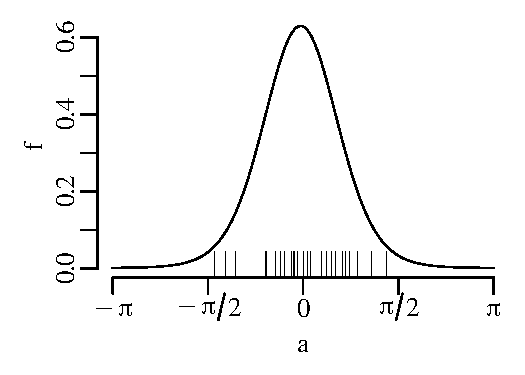
\includegraphics[width=\textwidth]{../figures/kappastriations.pdf}\medskip
\end{minipage}
\begin{minipage}[t][][t]{.6\textwidth}
  \captionof{figure}{Density plot and rug plot for the glacial
    striation data. The bell shaped density curve represents a von
    Mises distribution with concentration parameter $\kappa=2.8$ and
    mean $\mu=357.6^{\circ}$. In contrast with
    Figure~\ref{fig:vonMises}, in which the von Mises distribution was
    wrapped around a circle, here it is stretched out along a linear
    interval from $-\pi$ to $+\pi$.\medskip}
  \label{fig:kappastriations}
\end{minipage}

\section{Spherical data}
\label{sec:spherical-data}

The principles of directional statistics can be generalised from the
1-dimensional circular line in 2-dimensional space to a 2-dimensional
spherical surface in 3-dimensional space. The coordinates of data in
this space can be expressed as latitude ($l$) and longitude ($L$):
\begin{equation}
  \left\{
  \begin{split}
    x & = \cos[l]\sin[L]\\
    y & = \sin[l]\\
    z & = -\cos[l]\cos[L]
  \end{split}
  \right.
  \label{eq:lL}
\end{equation}

\noindent as strike (S) and dip (D):
\begin{equation}
  \left\{
  \begin{split}
    x & = -\cos[D]\sin[S]\\
    y & = \cos[D]\cos[S]\\
    z & = \sin[D]
  \end{split}
  \right.
  \label{eq:SD}
\end{equation}

\noindent or as azimuth (A) and dip (D):
\begin{equation}
  \left\{
  \begin{split}
    x & = \cos[D] \cos[A]\\
    y & = \cos[D] \sin[A]\\
    z & = \sin[D]
  \end{split}
  \right.
  \label{eq:AD}
\end{equation}

\noindent where the $x$-axis points towards the north, the $y$-axis
towards the east, and the $z$-axis points downwards.  Spherical data
can be visualised on a 2-dimensional surface by stereographic map
projection, using either a Wulff equal angle or a Schmidt equal area
\textbf{stereonet}:

\noindent\begin{minipage}[t][][b]{.6\textwidth}
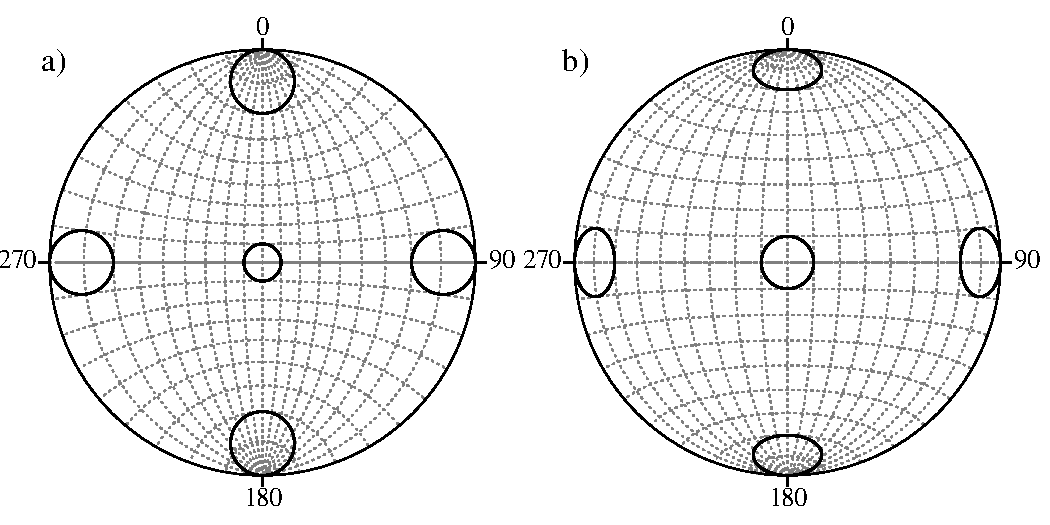
\includegraphics[width=\textwidth]{../figures/wulffschmidt.pdf}\medskip
\end{minipage}
\begin{minipage}[t][][t]{.4\textwidth}
  \captionof{figure}{a) Wulff equal angle and b) Schmidt equal area
    stereonets, with circles of $10^{\circ}$ radius drawn at azimuths
    of $0^{\circ}, 90^{\circ}, 180^{\circ}$ and $270^{\circ}$, and
    dips of $10^{\circ}$ and $90^\circ$. As the names suggest, the
    Wulff equal angle net preserves the shape of the circles, and the
    Schmidt equal area net their size.\medskip}
  \label{fig:wulffschmidt}
\end{minipage}

The Wulff net is used in structural geology and the Schmidt net in
crystallography. Given the Cartesian coordinates $\{x,y,z\}$, the
stereographic projection proceeds as follows:
\begin{equation}
  \left\{
  \begin{split}
    X & = \tan(\phi) \sin(\theta) \\
    Y & = \tan(\phi) \cos(\theta)
  \end{split}
  \right.
\end{equation}

\noindent for the Wulff net, and 
\begin{equation}
  \left\{
  \begin{split}
    X & = \sqrt{2}\sin(\phi)\sin(\theta) \\
    Y & = \sqrt{2}\sin(\phi)\cos(\theta)
  \end{split}
  \right.
\end{equation}

\noindent for the Schmidt net, where
\begin{equation}
  \left\{
  \begin{split}
    \phi & = \arccos\left(\sqrt{{x^2+y^2+(z-1)^2}}/{2}\right) \\
    \theta & = \mbox{arctan2}\left({x},{y}\right)
  \end{split}
  \right.
\end{equation}

Stereonets can be used to visualise

\begin{enumerate}

\item geographical data:

\noindent\begin{minipage}[t][][b]{.6\linewidth}
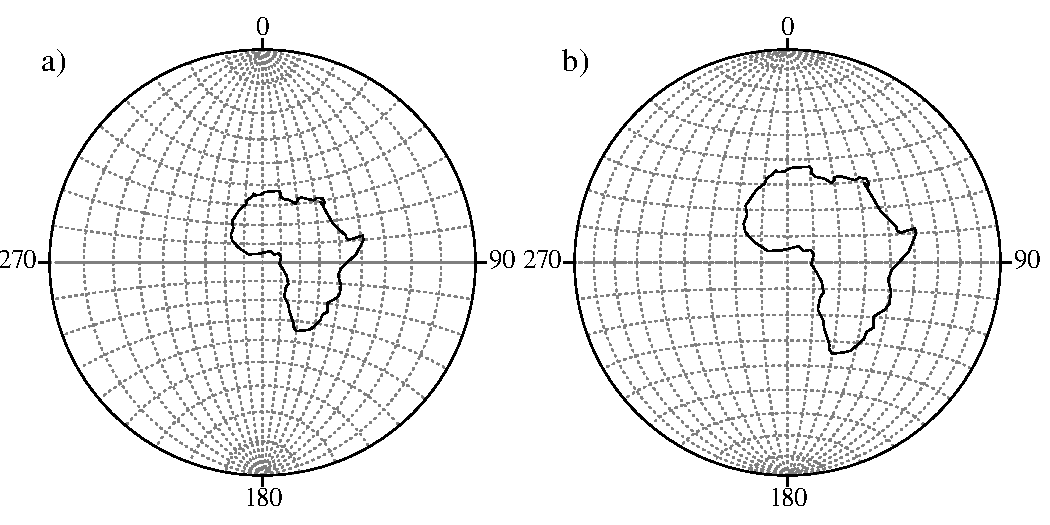
\includegraphics[width=\textwidth]{../figures/Africa.pdf}\medskip
\end{minipage}
\begin{minipage}[t][][t]{.4\linewidth}
  \captionof{figure}{a) Wulff and b) Schmidt projection of the African
    continent.  The Wulff net shows Africa in its right shape, and the
    Schmidt net shows it at the right size. No two dimensional
    projection can achieve both goals at once.\medskip}
  \label{fig:Africa}
\end{minipage}

\item palaeomagnetic data, such as the following dataset of 10
  declination (= azimuth) and inclination (= dip) measurements:

\begin{tabular}{c|cccccccccc}
declination & 47.9 & 46.3 & 44.7 & 50.9 & 56.4 & 42.6 & 44.9 & 41.5 & 47.9 & 39.6 \\
inclination & 28.6 & 20.1 & 15.6 & 18.1 & 17.5 & 28.7 & 12.2 & 24.5 & 20.6 & 15.0 \\
\end{tabular}

\noindent\begin{minipage}[t][][b]{.3\linewidth}
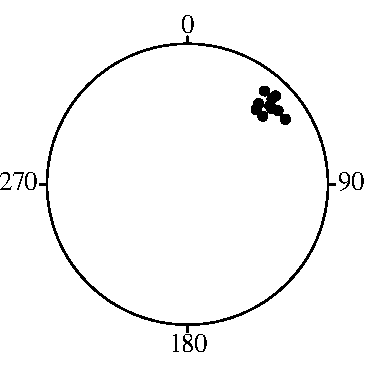
\includegraphics[width=\textwidth]{../figures/palaeomag.pdf}\medskip
\end{minipage}
\begin{minipage}[t][][t]{.7\linewidth}
  \captionof{figure}{The palaeomagnetic declination (=azimuth) and
    inclination (=dip) of 10~samples shown in a Schmidt equal area
    diagram.\medskip}
  \label{fig:palaeomag}
\end{minipage}

\item structural measurements, such as this set of 10 strikes and dips
  on a fault plane:

\begin{tabular}{c|cccccccccc}
strike & 226 & 220 & 223 & 222 & 233 & 227 & 234 & 229 & 227 & 224 \\
dip & 28.4 & 35.3 & 41.0 & 39.6 & 48.3 & 34.7 & 34.5 & 36.0 & 34.2 & 28.7
\end{tabular}  

\noindent\begin{minipage}[t][][b]{.3\linewidth}
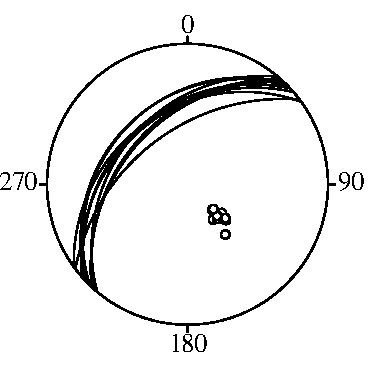
\includegraphics[width=\textwidth]{../figures/fault.pdf}\medskip
\end{minipage}
\begin{minipage}[t][][t]{.7\linewidth}
  \captionof{figure}{10 fault plane measurements shown on a Wulff
    stereonet. The white circles mark the `pole' of the planar
    measurements, i.e. a perpendicular line to the plane. The circular
    segments mark the intersection of the planes with bottom half of a
    sphere, shown in an equal angle projection.\medskip}
  \label{fig:fault}
\end{minipage}

\end{enumerate}

\section{Spherical distributions}
\label{sec:spherical-distributions}

The statistical analysis of spherical data is similar to that of the
circular data in Sections~\ref{sec:circular} and
\ref{sec:circular-distributions}. The von Mises -- Fisher (vMF)
distribution generalises the von-Mises distribution of
Equation~\ref{eq:vonMises}.  In three dimensions, the density function
for the vMF distribution is given by:
\begin{equation}
  f(\{x,y,z\}|\{\mu_x,\mu_y,\mu_y\},\kappa) = \frac{\kappa\exp[\kappa
      (x\mu_x+y\mu_y+z\mu_z)]}{2\pi(\exp[\kappa]-\exp[-\kappa])}
  \label{eq:vonMisesFisher}
\end{equation}

\noindent where $\mathbf{\mu}=\{\mu_x,\mu_y,\mu_z\}$ is a unit vector
representing the mean of the distribution in Cartesian coordinates,
and $\kappa$ is the concentration parameter. $\mathbf{\mu}$ and
$\kappa$ are unknown but can be estimated from the data using the
vector sum. To average a collection of $n$ spherical measurements:
\begin{equation}
  \left\{\bar{x},\bar{y},\bar{z}\right\} =
  \left\{\sum_{i=1}^{n}\frac{x_i}{n\bar{R}},
  \sum_{i=1}^{n}\frac{y_i}{n\bar{R}},
  \sum_{i=1}^{n}\frac{z_i}{n\bar{R}}
  \right\}
  \label{eq:3Dvectormean}
\end{equation}

\noindent where $\{x_i,y_i,z_i\}$ are the Cartesian coordinates
computed using Equation~\ref{eq:lL}, \ref{eq:SD} or \ref{eq:AD},
and $\bar{R}$ is the concentration parameter:
\begin{equation}
  \bar{R} = \frac{1}{n}
    \sqrt{\left(\sum_{i=1}^{n}x_i\right)^2 +
      \left(\sum_{i=1}^{n}y_i\right)^2 +
      \left(\sum_{i=1}^{n}z_i\right)^2
    }
\end{equation}

\noindent which is related to the (approximate) value for $\kappa$ by
Equation~\ref{eq:kappa} (with $p=2$).

Then the average latitude and longitude are given by:
\begin{equation}
  \left\{
  \begin{split}
  \bar{L} & = \mbox{arctan2}\left(-\bar{x},\bar{z}\right)\\
  \bar{l} & = \arcsin\left(\bar{y}\right)
  \end{split}
  \right.
\end{equation}

\noindent the average strike and dip:
\begin{equation}
  \left\{
  \begin{split}
    \bar{S} & = \mbox{arctan2}\left(-\bar{x},\bar{y}\right)\\
    \bar{D} & = \arcsin\left(\bar{z}\right)
  \end{split}
  \right.
\end{equation}

\noindent and the average azimuth and dip:
\begin{equation}
  \left\{
  \begin{split}
    \bar{D} & = \mbox{arctan2}\left(\bar{y},\bar{x}\right)\\
    \bar{A} & = \arcsin\left(\bar{z}\right)
  \end{split}
  \right.
\end{equation}

Applying this procedure to the palaeomagnetic and structural datasets:

\noindent\begin{minipage}[t][][b]{.6\textwidth}
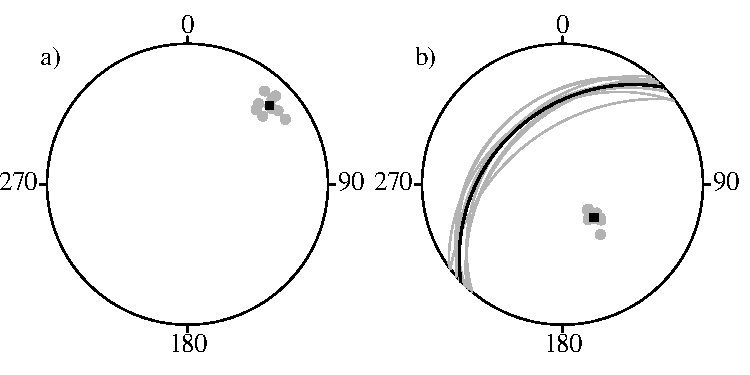
\includegraphics[width=\textwidth]{../figures/sphericalmean.pdf}
\end{minipage}
\begin{minipage}[t][][t]{.4\textwidth}
  \captionof{figure}{a) the palaeomagnetic data of
    Figure~\ref{fig:palaeomag} shown in grey, with their vector mean
    marked as a black square. b) the fault data of
    Figure~\ref{fig:fault} in grey with the vector mean as a black
    square and great circle, respectively.\medskip}
  \label{fig:sphericalmean}
\end{minipage}

\section{Orientations}\label{sec:orientations}

It is important to make a distinction between \emph{directions} such
as `north' or `east' and \emph{orientations} such as `north--south'
and `east-west'. The glacial striations of Section~\ref{sec:circular}
are a clear example of directional data: on average, the striations
point towards the north, suggesting a southerly ice source.  In
contrast, consider the following dataset of 20 pebble orientations on
a beach:

\begin{center}
\begin{tabular}{ccccccccccccccc}
  32 & 33 & 34 & 37 & 40 & 41 & 42 & 43 & 45 & 53 \\
  210 & 212 & 214 & 217 & 220 & 221 & 222 & 223 & 226 & 230
\end{tabular}
\end{center}

Unlike the striations, there are not one but two ways to measure the
pebble orientations. For example, an angle of 45$^\circ$ degrees is
equivalent to an angle of 225$^\circ$. However, the vector mean
(Equation~\ref{eq:averagedirection}) assumes that they are distinct
angles. This can produce nonsensical results:

\noindent\begin{minipage}[t][][b]{.25\textwidth}
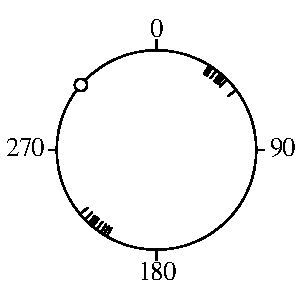
\includegraphics[width=\textwidth]{../figures/pebbles.pdf}\medskip
\end{minipage}
\begin{minipage}[t][][t]{.75\textwidth}
  \captionof{figure}{20 pebbles in a sedimentary bed are aligned in a
    NE--SW direction. Half of the measurements were recorded as
    northeasterly and the other half as southwesterly. Both of angles
    are equivalent. The white circle marks the vector mean, which
    points in a southeasterly direction.\medskip}
  \label{fig:pebbles}
\end{minipage}

A better way to average orientational data is to maximise the
\textbf{moment of inertia}. Suppose that the circle of
Figure~\ref{fig:pebbles} is a ring, and that the tick marks have a
physical weight attached to them. If we were to spin this ring around
the y-axis, the it would wobble significantly. The wobble can be
eliminated by changing the spin axis to the direction that minimises
the moment of inertia of the spinning ring.

\noindent\begin{minipage}[t][][b]{.25\textwidth}
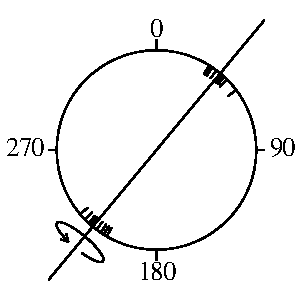
\includegraphics[width=\textwidth]{../figures/inertia.pdf}\medskip
\end{minipage}
\begin{minipage}[t][][t]{.75\textwidth}
  \captionof{figure}{The diagonal line tilts at an angle of
    40$^\circ$.  It marks the direction that minimises the moment of
    inertia of a circle with point masses attached to the angular
    measurements marked by the radial ticks. If the circle and the
    point masses were spun around this line, then they would do so
    without wobbling. The same is true for the perpendicular
    direction, which maximises the moment of inertia.\medskip}
  \label{fig:inertia}
\end{minipage}

The moment of inertia can be minimised by calculating the Cartesian
coordinates of the angular data, and calculating their covariance
matrix:

\begin{equation}
  \begin{split}
  \Sigma = &
  \left[
    \begin{array}{@{}cc@{}}
      s_x^2 & s_{x,y} \\
      s_{y,x} & s_y^2
    \end{array}
    \right] =
  \left[
    \begin{array}{@{}cc@{}}
      \frac{1}{n}\sum\limits_{i=1}^{n} (x_i-0)^2 & 
      \frac{1}{n}\sum\limits_{i=1}^{n} (x_i-0)(y_i-0) \\
      \frac{1}{n}\sum\limits_{i=1}^{n} (y_i-0)(x_i-0) &
      \frac{1}{n}\sum\limits_{i=1}^{n} (y_i-0)^2
    \end{array}
    \right] \\
  ~ & =
  \frac{1}{n}
  \left[
    \begin{array}{@{}cc@{}}
      \sum\limits_{i=1}^{n} x_i^2 & 
      \sum\limits_{i=1}^{n} x_iy_i \\
      \sum\limits_{i=1}^{n} x_iy_i &
      \sum\limits_{i=1}^{n} y_i^2
    \end{array}
    \right] =
  \sum\limits_{i=1}^{n}
  \left[
    \begin{array}{@{}c@{}}
      x_i \\ y_i
    \end{array}
    \right]
  \left[
    \begin{array}{@{}cc@{}}
      x_i & y_i
    \end{array}
    \right]
  \end{split}
  \label{eq:sphericalsigma}
\end{equation}

For the pebble data:
\[
\Sigma =
\left[
  \begin{array}{@{}cc@{}}
    0.62 & 0.51 \\
    0.51 & 0.44
  \end{array}
  \right]
\]
    
Subjecting their covariance matrix to an eigendecomposition (see
Equation~\ref{eq:eigen}) yields two eigenvalues and eigenvectors:
\[
\Sigma = Q \Lambda Q^{-1} =
\left[
  \begin{array}{@{}cc@{}}
    -0.77 & 0.64 \\
    -0.64 & -0.77
  \end{array}
  \right]
\left[
  \begin{array}{@{}cc@{}}
    0.989  & 0 \\
    0 & 0.011
  \end{array}
  \right]
\left[
  \begin{array}{@{}cc@{}}
    -0.77 & -0.64 \\
    0.64 & -0.77
  \end{array}
  \right]
\]

The first eigenvector defines a direction of $\bar{\theta} =
\mbox{atan}(-0.64/-0.77) = 0.70 = 40^\circ$ (see
Figure~\ref{fig:inertia}). It accounts for 98.9\% of the data
variance, as indicated by the first eigenvalue.\medskip

The same procedure can be used to average orientational data on a
sphere. For example, consider a structural dataset for a subhorizontal
bed. Suppose that some measured surfaces dip gently to the north and
others gently to the south:

\begin{center}
  \begin{tabular}{c|cccccccccc}
    strike & 77.1 & 94.9 & 73.2 & 122.8 & 97.3 &
    254.7 & 280.4 & 285.6 & 282.5 & 264.0 \\
    dip & 5.6 & 1.9 & 10.1 & 7.8 & 3.2 & 0.0 & 8.5 & 2.3 & 3.4 & 6.7
\end{tabular}
\end{center}

Calculating the vector mean with Equation~\ref{eq:3Dvectormean} yields
a nonsensical (subvertical!) result:\medskip

\noindent\begin{minipage}[t][][b]{.35\textwidth}
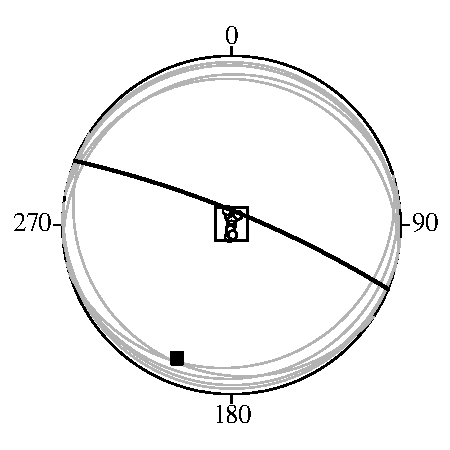
\includegraphics[width=\textwidth]{../figures/subhorizontal.pdf}
\end{minipage}
\begin{minipage}[t][][t]{.65\textwidth}
  \captionof{figure}{Open circles and grey lines shows 20 strike and
    dip measurements of a subhorizontal bed. The vector mean of these
    measurements is shown as a filled square and black line. It is
    perpendicular to the bed, which is clearly wrong. The large open
    square marks the direction that minimises the moment of inertia of
    the poles. This is a much more sensible orientational
    average.\medskip}
  \label{fig:subhorizontal}
\end{minipage}

The moment of inertia can be minimised for spherical data by
generalising Equation~\ref{eq:sphericalsigma} from two to three
dimensions and subjecting the resulting covariance matrix to an
eigendecomposition.
